The main idea of this algorithm is to compute a thin diagonal strip. Indeed, we can note that if the chains are quite similar the best alignment will not deviate too far from the diagonal. Thus, the idea of computing only a thin diagonal strip, assuming that the values outside this area are infinite.
We can use the algorithm described in class and using divide and conquer to compute the alignments only inside this diagonal strip (see figure 1 for an example).


This algorithm provides us with a solution that may not be optimal if the strip is too thin ; the width of the strip is called $w$. But we can note that the distance we get with this heuristic (let's call it $d_{h}$) is an upper-bound of the real distance (i.e. the distance obtained with the perfect alignment). Therefore we can build something stronger than a simple heuristic in the following way :
\begin{itemize}
	\item if $d_{h}\leqslant w$, then we know that the global alignment we got is the perfect one,
	\item otherwise to get the perfect global alignment we only have to run this algorithm a second time with a strip width of $w'=d_{h}$
\end{itemize}

With this algorithm, our space complexity is still linear in $n$. Our running time is decreased : if we only want an upper-bound, the running-time is $O(wn)$ whereas if we want the perfect solution the running time is bounded by $max(wn,d_{h(w)}n)$.
Therefore when we want the exact solution, we have to choose wisely $w$. Last, it is interesting to note that the more similar the two chains are, the better our algorithm performs.
\begin{figure}[H]
	\centering
		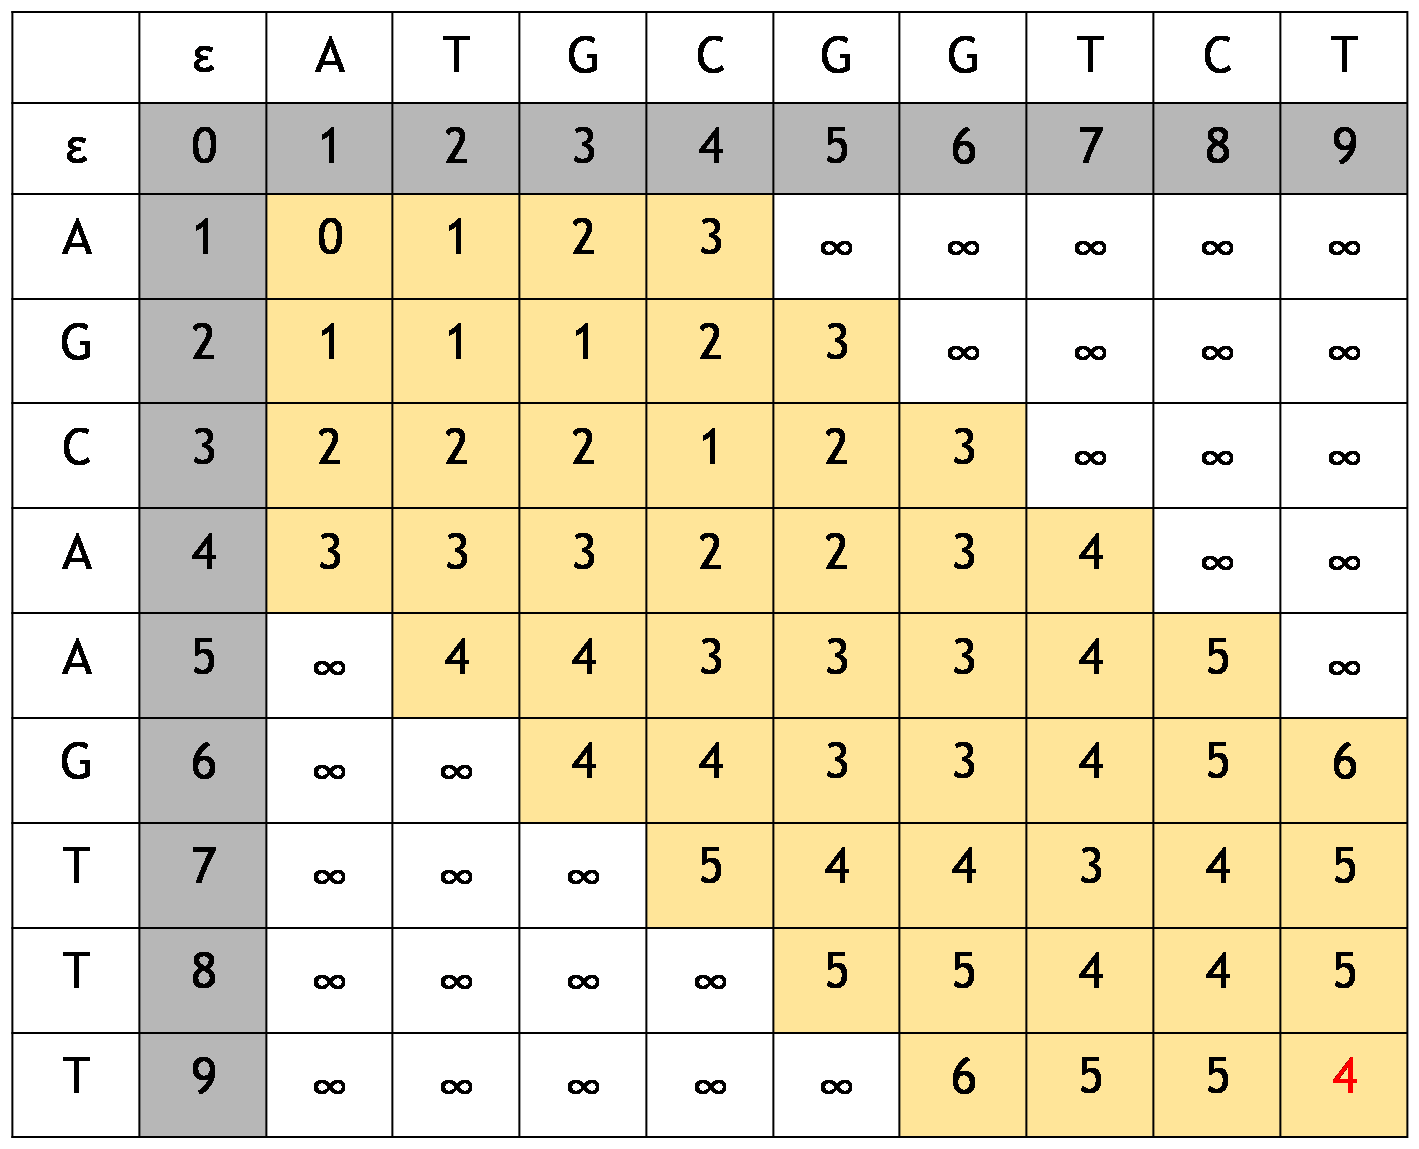
\includegraphics[height=7cm]{adn3.png}
	\caption{Illustration of our diagonal strip algorithm}
	\label{fig:adn}
\end{figure}
